\documentclass[eng,oneside]{mgr}
\usepackage{polski}
\usepackage[utf8]{inputenc}
\usepackage[T1]{fontenc}
\usepackage{graphicx}
\graphicspath{ {c:/użytkownicy/nieop/Pulpit} }
\usepackage{subfigure}
\usepackage{subfig}
\usepackage{psfrag}
\usepackage{amsmath}
\usepackage{amsfonts}
\usepackage{supertabular}
\usepackage{array}
\usepackage{tabularx}
\usepackage{hhline}
\usepackage{showlabels}

\title{Rozpoznawanie znaków tekstowych drogowych w systemie osób niewidomych}
\engtitle{The text road signs recognition in the system of blind people}
\author{Karolina Raczyńska}
\supervisor{dr inż. Łukasz Jeleń}
\date{09.12.2016}
\field{Automatyka i Robotyka (AIR)}
\specialisation{Technologie Informacyjne w Automatyce (ART)}
\begin{document}
\maketitle
\tableofcontents 
\chapter{Wstęp}
\section{Cel pracy}
\section{Zakres pracy}
\chapter{Przetwarzanie obrazu}
\hspace{1cm} Obraz to między innymi źródło informacji - nie tylko wzrokowej. Aby uzyskać dane, które są w nim zapisane, należy go odpowiednio przetworzyć. W dziedzinie nauki, jaką jest przetwarzanie obrazów, wyróżniamy kilka etapów działania. Uproszczony schemat został przedstawiony na rysunku poniżej.
\begin{figure}[htbp]
\centering
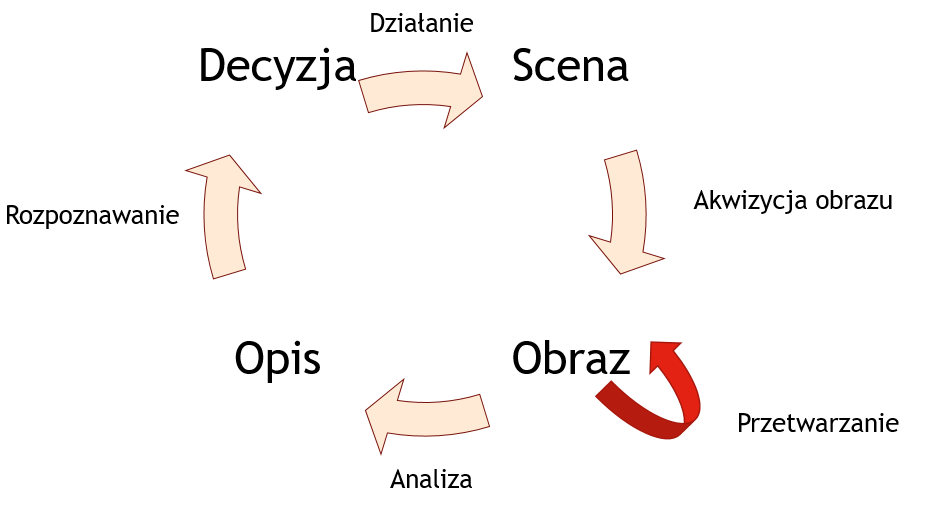
\includegraphics[scale=0.5]{cyklprzetwarzania.png}
\caption{Schemat cyklu przetwarzania obrazu.}\par\medskip
\end{figure}
\hspace{1cm} Poniżej zostały omówione poszczególne etapy.
\begin{enumerate}
\item 	Akwizycja obrazu – zamiana energii świetlnej od każdej punktu sceny na sygnał elektryczny, czyli zbieranie danych o każdym pikselu. Scena jaką obserwujemy jest funkcją ciągłą, przy przetwarzaniu jej na obraz cyfrowy, pewna część danych zostaje stracona. Typowo korzysta się z dwóch sposobów pozyskiwania sygnały dyskretnego z sygnału ciągłego i jest to: kwantyzacja oraz próbkowanie. Kwantyzacja jest to pobieranie danych w funkcji wartości funkcji – w zależności od niej przyporządkowuje się próbkę do odpowiedniego przedziału, czyli kwantu, natomiast próbkowanie polega na zbieraniu danych w funkcji czasu.
\item 	Przetwarzanie obrazu – zmniejszenie obrazu, eliminacja zakłóceń, filtracja wstępna, której celem jest wyeksponowanie na obrazie ważnych cech, takich jak krawędzie lub duże jednokolorowe obiekty. Do tego celu stosuje się np. transformację obrazu kolorowego na skalę odcieni szarości, tudzież na bitmapę składającą się jedynie z dwóch wartości.
\item 	Analiza obrazu – wydobycie wcześniej wyeksponowanych cech, w celu ich późniejszego rozpoznania, już nie jako kształtu ale jako konkretnej informacji. Wynikiem tego etapu nie jest już obraz, a dane w postaci liczbowej lub statystycznej.
\item 	Decyzja – rozpoznanie obrazu, zanalizowanie cech, pozyskanie informacji, a przede wszystkim klasyfikacja$\cite{obrazy}$.
\end{enumerate}
\hspace{1cm} Wszystkie te etapy dzieją się w systemie wizyjnym do którego można zaliczyć np. komputer, telefon, aparat fotograficzny, a do jego podstawowych funkcji należy:
\begin{itemize}
\item Przyjęcie obrazu,
\item zapisanie obrazu,
\item właściwa obróbka obrazu,
\item wyświetlenie obrazu$\cite{wizja}$;
\end{itemize}

\section{Przetwarzanie do skali szarości}
\hspace{1cm} RGB, jest modelem przestrzeni barw, w którym każdy piksel opisują trzy wartości: intensywność koloru czerwonego, intensywność koloru zielonego oraz intensywność koloru niebieskiego. Obraz w odcieniach szarości to obraz w którym procentowy udział każdej z tych trzech instancji jest równy. Aby uzyskać taki wynik należy przeprowadzić pewne modyfikacje na wartościach pikseli. Najbardziej znane są trzy algorytmy:
\begin{itemize}
\item Lekkość (ang. Lightness) – metoda ta polega na tym, że z trzech wartości: intensywności koloru czerwonego, zielonego oraz niebieskiego w pikselu, zostaje wybrana wartość największa oraz najmniejsza, a wynikiem transformacji jest średnia arytmetyczna tych dwóch wartości.
\\
\begin{equation}
p=\frac{max(R,G,B) + min(R,G,B)}{3}
\end{equation}
\item Średnia (ang. Average) – metoda ta, najprostsza, dzieli sumę wartości intensywności trzech kolorów przez trzy.
\\
\begin{equation}
p=\frac{R + G + B}{3}
\end{equation}
\item Jasność (ang. Luminance) – metoda również opierająca się na średniej, ale w tym wypadku jest to średnia ważona. Ludzki wzrok jest najbardziej czuły na kolor zielony, właśnie dlatego intensywność zieleni ma największą wagę. Wyjściowy piksel przyjmuje wartość:
\\
\begin{equation}
p=\frac{0.21R + 0.72G + 0.07B}{3}\cite{grayscale}
\end{equation}

\end{itemize}
\section{Binaryzacja}
\hspace{1cm} Binaryzacja to operacja punktowa. Wynikiem tej operacji jest obraz binarny, czyli taki, w którym każdy z pikseli przyjmuje tylko jedną z dwóch wartości. Ideą tego zabiegu jest wyodrębnienie obiektu od tła przez nadanie pikselom tych dwóch instancją różnych wartości. Wejściowym obrazem jest zazwyczaj obraz przetworzony do skali szarości, którego piksele przyjmują wartości od 0 do 255. Najczęściej stosowaną metodą klasyfikacji piksela do jednej z dwóch klas jest progowanie – sprawdzenie czy wartość piksela przekracza zadany próg czy też nie i w zależności od wyniku tego zdania logicznego – przypisanie odpowiedniej wartości. Ważnym zagadnieniem tego sposobu jest celne dobranie progu. Najbardziej intuicyjnym rozwiązaniem byłoby wybranie środkowej wartości z przedziału skali wartości zadanego obrazu. Jest to rozwiązanie globalne, sprawdzające się w przypadku gdy tło jest wyraźnie jaśniejsze lub ciemniejsze od pozostałych obiektów sceny w każdej z jej współrzędnych, a liczba pikseli tła jest w przybliżeniu równa liczbie pikseli reszty elementów. Dlatego szuka się optymalnych wartości progu i wykorzystuje się do tego takie metody jak opisana poniżej metoda Otsu.
\subsection{Metoda Otsu}
\hspace{1cm} Metoda Otsu należy do rodziny metod optymalnych względem pewnej funkcji kryterialnej. W tym przypadku ową funkcja kryterialną jest wariancja wewnątrzklasowa oraz międzyklasowa. Metoda ta jest bardzo prosta, w uogólnieniu używa momentów zerowego oraz pierwszego stopnia histogramu obrazu.
Pierwszym etapem poszukiwania wartości progowej metodą Otsu jest normalizacja histogramu obrazu w skali szarośic. Zakłada się, że piksele przyjmują wartości z L poziomów, a do każdego i-tego poziomu jest przydzielana ni liczba pikseli. Przyjmując, że N to liczba wszystkich pikseli obrazu, rozkład prawdopodobieństwa tego histogramu przedstawiony jest następująco:
\\ 
\begin{equation}
 p_i = \frac{n_i}{N} \hspace{1cm}
 p_i \geq 0, \sum_{i=1}^L p_i = 1 
\end{equation}
\\ 
\hspace{1cm} Następnym krokiem jest dychotomia pikseli, czyli podział wszystkich elementów na dwie klasy względem pewnego progu t. Wtenczas pikseli, które przyjmują wartości mniejsze od zadanej wartości progowej t zostaną sklasyfikowane do klasy $K_0$, a te większe do klasy $K_1$. Wtedy prawdopodobieństwo tego, że badany piksel zostanie przypisany do danej klasy jest określone wzorami:
\\
\begin{equation}
\omega_0 = Pr(K_0)=\sum_{i=1}^t p_i = \omega(t)\hspace{1cm}
\end{equation}
\
\begin{equation}
\omega_1 = Pr(K_1)=\sum_{i=t+1}^L p_i = 1 - \omega(t)
\end{equation}
\\
\hspace{1cm} Średnia wartość piksela przyjmowana w klasie określona została w poniższych wzorach:
\\
\begin{equation}
\mu_0=\sum_{i=1}^t Pr(i|K_0)=\sum_{i=1}^t \frac{ip_i}{\omega_0}=\frac{\mu(t)}{\omega(t)}
\end{equation}
\
\begin{equation}
\mu_1=\sum_{i=t+1}^L iPr(i|K_1)=\sum_{i=t+1}^L \frac{ip_i}{\omega_1} = \frac{\mu_T-\mu(t)}{1-\omega(t)}
\end{equation}
\\
\hspace{1cm} Gdzie:
\\
\begin{equation}
\omega(t)=\sum_{i=1}^t p_i
\end{equation}
\
\begin{equation}
\mu(t)=\sum_{i=1}^t ip_i
\end{equation}
\\
\hspace{1cm} Powyższe wartości są skumulowanymi momentami zerowego oraz pierwszego stopnia obrazu dla wartości progowej równej t. A średnia z wartości pikseli na całym obrazie może zostać zapisane wzorem:
\\
\begin{equation}
\mu_T = \mu(L) = \sum_{i=1}^L ip_i
\end{equation}
\hspace{1cm} Niezależnie od wyboru wartości parametru t, prawdziwe są równania:
\\
\begin{equation}
\omega_0\mu_0+\omega_1\mu_1=\mu_T, \hspace{1cm} \omega_0+\omega_1=1. 
\end{equation}
\\
\hspace{1cm} Wariancje obu klas można przedstawić następująco:
\\
\begin{equation}
\sigma_0^{2}=\sum_{i=1}^t {(i-\mu_0)}^2 Pr(i|K_0)=\sum_{i=1}^t {(i-\mu_0)}^2 \frac{p_i}{\omega_0}
\end{equation}
\
\begin{equation}
\sigma_0^{2}=\sum_{i=t+1}^t {(i-\mu_1)}^2 Pr(i|K_1)=\sum_{i=t+1}^L {(i-\mu_1)}^2 \frac{p_i}{\omega_1}
\end{equation}
\\
\hspace{1cm} W kolejnym etapie należy sprawdzić czy wartość zmiennej k jest wartością optymalną względem funkcji kryterialnej. Funkcją kryterialną, jak wcześniej wspomniano jest:
\begin{itemize}
\item Wariancja wewnątrz klasowa, dąży do minimalizacji,
\begin{equation}
\lambda=\frac{\sigma_B^2}{\sigma_W^2}, \hspace{0.5cm} \sigma_W^2 = \omega_0\sigma_0^2 + \omega_1\sigma_1^2, \hspace{0.5cm} \sigma_B^2 = \omega_0\omega_1{(\mu_1-\mu_2)}^2 
\end{equation}
\item Wariancja między klasowa, dąży do maksymalizacji.
\begin{equation}
\kappa=\frac{\sigma_T^2}{\sigma_W^2}, \hspace{0.5cm} \sigma_T^2 = \sum_{i=1}^L {(i-\mu_T)}^2 p_i 
\end{equation}
\end{itemize}
\hspace{1cm} Co intuicyjnie zgadza się z pożądanym efektem działania algorytmu. Chce się aby wartości pikseli w klasach były do siebie jak najbardziej zbliżone, a między klasami występowała jak największa różnica.
Kryterium jakie stosuje się do optymalizacji wartości k jest łączna wariancja poziomów $\eta$. Parametr jest optymalny, jeżeli $\eta$ przyjmuje wartość jak największą, tym samym wariancja wewnątrz klasowa. Wartość ta będzie zerowa jedynie w przypadku gdy wszystkie piksele obrazu zostaną zakwalifikowane tylko do jednej z klas, jednak jest to sprzeczne z celem działania algorytmu, więc w tym kontekście maksimum zawsze istnieje.
\begin{equation}
\eta=\frac{\sigma_B^2}{\sigma_T^2}, \hspace{0.5cm} 
\end{equation}
\hspace{1cm}Zaletą tej metody jest jej prostota – korzysta się jedynie z momentów zerowego i pierwszego rzędu, a także stabilność – optymalny próg jest wybrany automatycznie, nie bazuje na zróżnicowaniach (takich jak lokalne zbiory pikseli o niskich lub wysokich wartościach), skupia się na globalnych właściwościach obrazu, histogramie. Ważną cechą jest też uniwersalność metody, dzięki, której można ją wykorzystywać w różnych dziedzinach analizy obrazu. Może służyć do binaryzacji, jak wykorzystano w projekcie, wykorzystywana jest też przy progowaniu$\cite{binaryzacja}$.

\section{Wykrywanie krawędzi}
\hspace{1cm} Przetwarzanie obrazów opiera się na wydobywaniu z obrazu takich cech, które są istotne przy późniejszej analizie i identyfikacji obiektów na nim zawartych. Jedną z takich cech jest krawędź, czyli znaczna lokalna zmiana w intensywności obrazu, związana z brakiem ciągłości w intensywności obrazu lub w pierwszej pochodnej intensywności obrazu. Występują dwa rodzaje takiej zmiany ciągłości:
\begin{enumerate}
\item Nieciągłość skokowa - intensywność obrazu zmienia się z jednej wartości w drugą i przez jakiś czas tą wartość utrzymuje, przypomina odpowiedź skokową, na obrazie może być to moment styku dwóch obiektów;
\item Nieciągłość liniowa - intensywność obrazu zmienia się z jednej wartości w drugą lecz w krótkim okresie czasu do niej powraca, przypomina odpowiedź impulsową, na obrazie może to być przerwanie w obiekcie; 
\end{enumerate}
\hspace{1cm} W praktyce jednak tego typu krawędzie zdarzają się dość rzadko, krawędzie nie są aż tak wyraziste i skok przypomina bardziej rampę, a linia - dach$\cite{krawedz}$.
Wykrywanie krawędzi to przede wszystkim rozpoznawanie znacznych zmian w obrazie, jest to mocno związane z wyznaczaniem maksimum pierwszej pochodnej. 
\hspace{1cm} Gradient jest miarą zmiany, wektorem, który wskazuje kierunki i szybkość wzrostu wartości, to dwuwymiarowy odpowiednik pierwszej pochodnej. W obrazie zmianą jest różnica w intensywności koloru. To właśnie on jest bazą większości algorytmów wykrywających krawędzie. Gradient obrazu dany jest wzorem:
\begin{equation}
\nabla f = \binom{g_x}{g_y} = \binom{\frac{\delta f}{\delta x}}{\frac{\delta f}{\delta y}}
\end{equation} 
$g_x $- gradient w kierunku x,
\\
$g_y $- gradient w kierunku y
 \\
 \\
\hspace{1cm} Kierunek zmian można wyliczyć z poniższego wzoru:
\begin{equation}
\theta = \tan^{-1} \binom{g_x}{g_y}
\end{equation}

\hspace{1cm} Etapy wykrywania krawędzi:
\begin{enumerate}
\item Filtracja\\
Aby ulepszyć działanie detektora krawędzi należy pozbyć się szumów, które utrudniają wyliczanie gradientów. Należy jednak zachować umiar, zbyt duże wygładzanie obrazu może spowodować osłabienie krawędzi. Często w tym celu stosuje się rozmycie Gaussowskie, które zostało omówione szerzej w podrozdziale 2.3.1.
\item Wzmocnienie \\
W polach obrazu gdzie umiejscowione są największe zmiany intensywności koloru podkreśla się te piksele, które mają na tą zmianę największy wpływ. Używa się w tym celu gradientu.
\item Wykrycie\\
W związku z licznymi zanieczyszczeniami i szumami obecnymi na obrazie zdarza się, że piksele o niezerowym gradiencie nie należą do krawędzi. Aby pominąć piksele nieistotne, wybiera się próg wedle którego ocenia się czy piksel należy do krawędzi czy też nie.
\item Zlokalizowanie\\
Etap ten składa się na większość algorytmów, polega na określeniu rozdzielczości, położenia pikseli, które składają się na krawędź. Jest to zdecydowanie przydatne w momencie potrzeby wyodrębnienia z obrazu konkretnego obiektu\cite{etapy}.

\end{enumerate}

\subsection{Detektor Canny}
\hspace{1cm} Detektor ten jest najczęściej używanym detektorem w świecie przetwarzania obrazów. Należy do rodziny detektorów Gaussowskich, specjalizujących się w wykrywaniu krawędzi skokowych. Jest to algorytm optymalny względem kilku kryteriów:
\begin{itemize}
\item Poprawna detekcja - dąży się do minimalizacji klasyfikacji nieistniejących krawędzi jako krawędzi istniejących. Są większe szanse na pominięcie krawędzi niż na wykrycie krawędzi błędnej.
\item Poprawna lokalizacja - dąży się do tego, aby wykryte krawędzie znajdowały się jak najbliżej istniejących krawędzi.
\item Jednoznaczna odpowiedź - dąży się do minimalizacji lokalnych maksimów wokół wykrytej krawędzi, idea jest taka, aby dla każdego istniejącego punktu krawędzi zwracany był tylko jeden piksel.
\end{itemize}
\hspace{1cm} Sposób działania algorytmu można opisać w kilku krokach:
\begin{itemize}
\item [Krok 1] Obraz wejściowy należy poddać operacji rozmycia Gaussa, w celu pozbycia się szumów. Polega to na nałożeniu na obraz maski, która jest dyskretną aproksymacją funkcji Gaussa opisaną wzorem poniżej:
\begin{equation}
G(x,y) = \frac{1}{2\pi\sigma^2}e^{-\frac{x^2+y^2}{2\sigma^2}}
\end{equation}
\hspace{1cm} Matematycznie, nałożenie maski na obraz to wyliczenie splotu dyskretnych wartości funkcji Gaussa i pikseli obrazu\cite{gauss}.\\
\hspace{1cm} Rozmycie Gaussa jest zależne od wartości gradientu.
\item [Krok 2] Następnie wyliczona zostaje wartość oraz kierunek gradientu. 
\begin{equation}
gradient = \sqrt{G_x^2 + G_y^2} 
\end{equation}
\begin{equation}
\theta = \tan ^{-1} \frac{G_y}{G_x}
\end{equation}
\item [Krok 3] Wykrywa się punkty należące do krawędzi i tłumi te wartości, które nie są maksimami lokalnymi, aby pozbyć się niewyraźnych krawędzi.
\item [Krok 4]  W ostatnim etapie punkty krawędzi zostają połączone i wybiera się histerezę - przedział od najniższej wartości progu do najwyżej wartości progu w jakim ma się znaleźć krawędź. Najwyższy próg $k_{max}$ dotyczy mocnych krawędzi, natomiast najniższy próg $k_{min}$ dotyczy krawędzi słabych.
\end{itemize}
\chapter{Architektura systemu}
\chapter{Implementacja}
\chapter{Działanie aplikacji i testy}
\section {Wymagania wstępne}
\hspace{1cm} Aplikacja działa na smartfonach z oprogramowaniem Android o wersji SDK nie starszej niż 17. Wersją najbardziej oczekiwaną jest wersja 23. Smartfon musi posiadać aparat oraz ponad 13Mb wolnej pamięci – zostanie na niej zapisany folder – tessdata, z plikiem zawierającym dane potrzebne bibliotece Tess4j do przetwarzania obrazu w języku polskim. Język telefonu powinien być ustawiony na ten w jakim oczekiwane jest czytanie komunikatów przez aplikację. 
\section {Widok główny}
\begin{figure}[htbp]
\centering
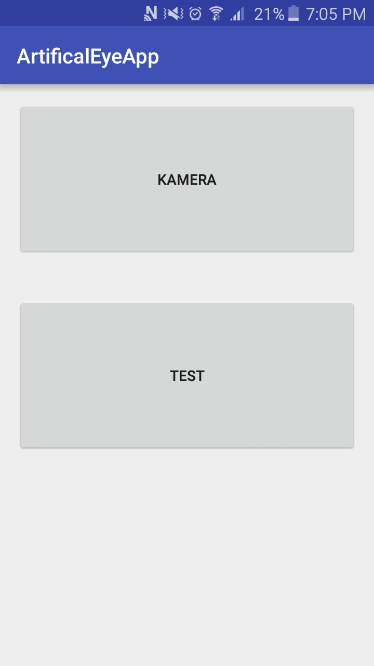
\includegraphics{glownywidok.png}
\caption{Główny widok aplikacji.}\par\medskip
\end{figure}
Jest to intuicyjny widok z dwoma dużymi przyciskami. Przy uruchomieniu aplikacji, informuje ona użytkownika komunikatem głosowym o położeniu przycisków i ich przeznaczeniu: „Kliknij na górze ekranu aby przejść do kamery – Kliknij na dole ekranu aby przejść do testów”. Aplikacja, poza widokiem głównym, posiada dwa widoki dodatkowe: użytkownika oraz testowy. Można się do nich dostać po wciśnięciu w odpowiedni przycisk. Przycisk „Kamera” przekierowuje użytkownika do widoku z kamery smartfona, natomiast przycisk „Test” przekierowuje do widoku testowego.
\section {Widok docelowy}
\hspace{1cm} Widok docelowy przenosi użytkownika do kamery zainstalowanej na urządzeniu na którym działa aplikacja. W tym momencie użytkownik ma możliwość kliknięcia w ekran i zrobienia fotografii. W zależności od rodzaju telefonu, kamera może poprosić o potwierdzenie przesłania zdjęcia do dalszej przeróbki, o czym aplikacja poinformuje komunikatem głosowym, z dokładnym umiejscowieniem odpowiedniego przycisku na ekranie, zdjęcie też może zostać od razu przesłane.
\section {Widok testowy}
\begin{figure}[htbp]
\centering
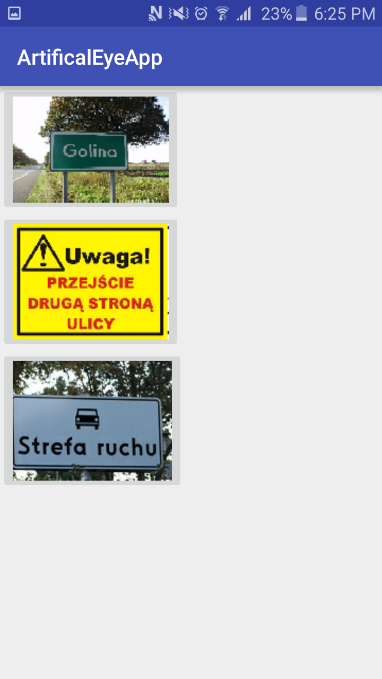
\includegraphics{widoktest.png}
\caption{Testowy widok aplikacji.}\par\medskip
\end{figure}
Osoba testująca, klikając na wybrane zdjęcie sprawia, że zostaje ono poddane przetwarzaniu. W efekcie końcowym otrzymuje się rozpoznany znak, wycięty ze zdjęcia, jako obraz binarny – zaprezentowany przez dwa odcienie – czarny oraz biały, kolory odwrócone, odpowiednio tak aby tekst był czarny, a tło białe, czyli obraz jaki na wejście otrzymuje algorytm rozpoznający tekst. Pod obrazem zostaje wyświetlony tekst, którzy otrzymano w wyniku działania biblioteki Tess4j. Zostaje on przeczytany przez aplikację, użytkownik może odtwarzać go dowolną liczbę razy, klikając na przycisk „Powiedz”. Poniżej, na zdjęciach numer 5.3, 5.4 oraz 5.5, zostały przedstawione wyniki działania aplikacji w trybie testowym.
\begin{figure}
\centering
\subfigure[Obraz przetwarzany.]{
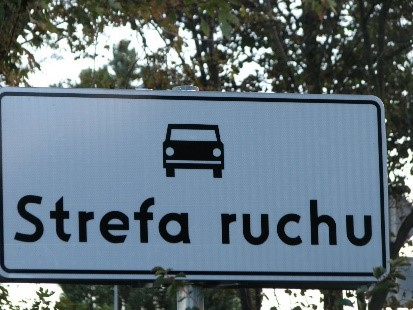
\includegraphics{strefaruchu.jpg}
}
\quad
\subfigure[Obraz przetworzony.]{
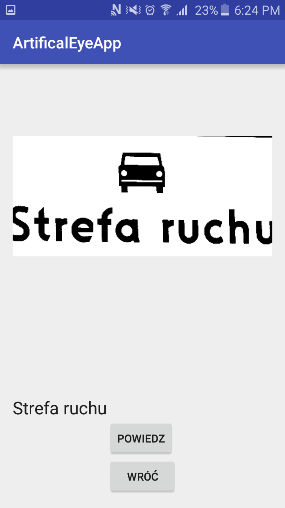
\includegraphics{strefaruchuwynik.png}
}
\caption{Wynik działania aplikacji.}
\end{figure}
\\
\begin{figure}
\centering
\subfigure[Obraz przetwarzany.]{

\includegraphics[scale=0.75]{uwaga.png}
}
\quad
\subfigure[Obraz przetworzony.]{

\includegraphics{uwagawynik.png}
}
\caption{Wynik działania aplikacji.}
\end{figure}

\begin{figure}
\centering
\subfigure[Obraz przetwarzany.]{
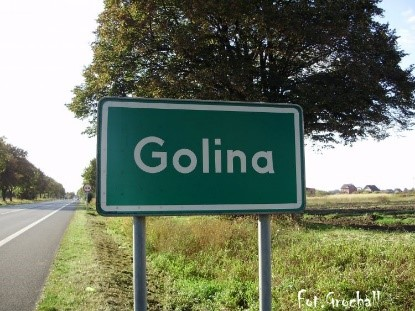
\includegraphics{golina.jpg}
}
\quad
\subfigure[Obraz przetworzony.]{
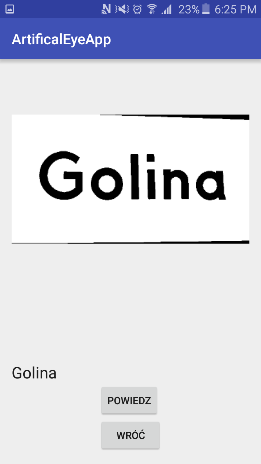
\includegraphics{golinawynik.png}
}
\caption{Wynik działania aplikacji.}
\end{figure}

\begin{thebibliography}{99}
\bibitem{obrazy} R. Tadeusiewicz, P. Korohoda: \emph{Komputerowa analiza i przetwarzanie obrazów}, wyd. Fundacji Postępu Telekomunikacji, ('3)
\bibitem{wizja} jw. ('5)
\bibitem{grayscale} http://www.johndcook.com/blog/2009/08/24/algorithms-convert-color-grayscale/
\bibitem{binaryzacja} http://web-ext.u-aizu.ac.jp/course/bmclass/documents/otsu1979.pdf
\bibitem{krawedz} R. Jain, R. Kasturi, B. G. Schunck, \emph{Machine Vision} McGraw-Hill, Inc., 1995 ('140)
\bibitem{etapy} jw. ('145-146)
\bibitem{gauss} http://homepages.inf.ed.ac.uk/rbf/HIPR2/gsmooth.htm
\end{thebibliography}
\end{document}
